\documentclass[letterpaper,12pt]{article}\usepackage[]{graphicx}\usepackage[]{color}
%% maxwidth is the original width if it is less than linewidth
%% otherwise use linewidth (to make sure the graphics do not exceed the margin)
\makeatletter
\def\maxwidth{ %
  \ifdim\Gin@nat@width>\linewidth
    \linewidth
  \else
    \Gin@nat@width
  \fi
}
\makeatother

\definecolor{fgcolor}{rgb}{0.345, 0.345, 0.345}
\newcommand{\hlnum}[1]{\textcolor[rgb]{0.686,0.059,0.569}{#1}}%
\newcommand{\hlstr}[1]{\textcolor[rgb]{0.192,0.494,0.8}{#1}}%
\newcommand{\hlcom}[1]{\textcolor[rgb]{0.678,0.584,0.686}{\textit{#1}}}%
\newcommand{\hlopt}[1]{\textcolor[rgb]{0,0,0}{#1}}%
\newcommand{\hlstd}[1]{\textcolor[rgb]{0.345,0.345,0.345}{#1}}%
\newcommand{\hlkwa}[1]{\textcolor[rgb]{0.161,0.373,0.58}{\textbf{#1}}}%
\newcommand{\hlkwb}[1]{\textcolor[rgb]{0.69,0.353,0.396}{#1}}%
\newcommand{\hlkwc}[1]{\textcolor[rgb]{0.333,0.667,0.333}{#1}}%
\newcommand{\hlkwd}[1]{\textcolor[rgb]{0.737,0.353,0.396}{\textbf{#1}}}%

\usepackage{framed}
\makeatletter
\newenvironment{kframe}{%
 \def\at@end@of@kframe{}%
 \ifinner\ifhmode%
  \def\at@end@of@kframe{\end{minipage}}%
  \begin{minipage}{\columnwidth}%
 \fi\fi%
 \def\FrameCommand##1{\hskip\@totalleftmargin \hskip-\fboxsep
 \colorbox{shadecolor}{##1}\hskip-\fboxsep
     % There is no \\@totalrightmargin, so:
     \hskip-\linewidth \hskip-\@totalleftmargin \hskip\columnwidth}%
 \MakeFramed {\advance\hsize-\width
   \@totalleftmargin\z@ \linewidth\hsize
   \@setminipage}}%
 {\par\unskip\endMakeFramed%
 \at@end@of@kframe}
\makeatother

\definecolor{shadecolor}{rgb}{.97, .97, .97}
\definecolor{messagecolor}{rgb}{0, 0, 0}
\definecolor{warningcolor}{rgb}{1, 0, 1}
\definecolor{errorcolor}{rgb}{1, 0, 0}
\newenvironment{knitrout}{}{} % an empty environment to be redefined in TeX

\usepackage{alltt}
\usepackage[top=1in,bottom=1in,left=1in,right=1in]{geometry}
\usepackage{setspace}
\usepackage[colorlinks=true,urlcolor=blue,citecolor=blue,linkcolor=blue]{hyperref}
\usepackage{indentfirst}
\usepackage{multirow}
\usepackage{booktabs}
\usepackage[final]{animate}
\usepackage{graphicx}
\usepackage{verbatim}
\usepackage{rotating}
\usepackage{tabularx}
\usepackage{array}
\usepackage{subfig} 
\usepackage[noae]{Sweave}
\usepackage{cleveref}
\usepackage[figureposition=bottom]{caption}
\usepackage{paralist}
\usepackage{acronym}
\usepackage{outlines}

%acronyms
\acrodef{doc}[DoC]{depth of colonization}
\acrodef{GIS}{Geographic Information System}

%knitr options


\IfFileExists{upquote.sty}{\usepackage{upquote}}{}
\begin{document}

\setlength{\parskip}{5mm}
\setlength{\parindent}{0in}

\title{Installing R and Optional RStudio}
\author{Marcus W. Beck}
\maketitle

\section{Installing R}

R is quickly becoming the statistical software of choice for researchers and analysts in a variety of disciplines.  In recent years, it has surpassed many commonly used statistical programs in both number of users and availability of statistical methods.  A fundamental difference between R and other statistical software packages is that R is open-source, meaning it is both free for download and the source code is available under the \href{http://www.gnu.org/licenses/gpl-2.0.html}{GNU General Project License}.  Anyone can contribute new techniques or analytical methods, which has been a primary factor enabling the growth of R.  These contributions are called `packages'.  Currently, almost 6000 packages are available for R.   

Installing R is straightforward.  The source binaries (i.e., installation files) are available at \href{http://www.r-project.org}{www.r-project.org}.  Note that installation will require administrative privileges.  After successful installation, all packages that have been developed as supplementary to those included in the base installation can be installed without administrative rights.  Because R is open source, the source binaries and supporting packages are not hosted in a single location.  Before the files are downloaded, a mirror where the files are hosted must be chosen.  Additional package installations will also require selecting a mirror.  The mirror is part of CRAN, or Centralized R Archive Network, which is a network of all available locations that have the R source files and packages.  The following is a step-by-step guide to installing R through this network.  Package installation will be covered later.

\begin{enumerate}

\item{Visit the R website using a web browser: \href{http://www.r-project.org}{www.r-project.org}.}

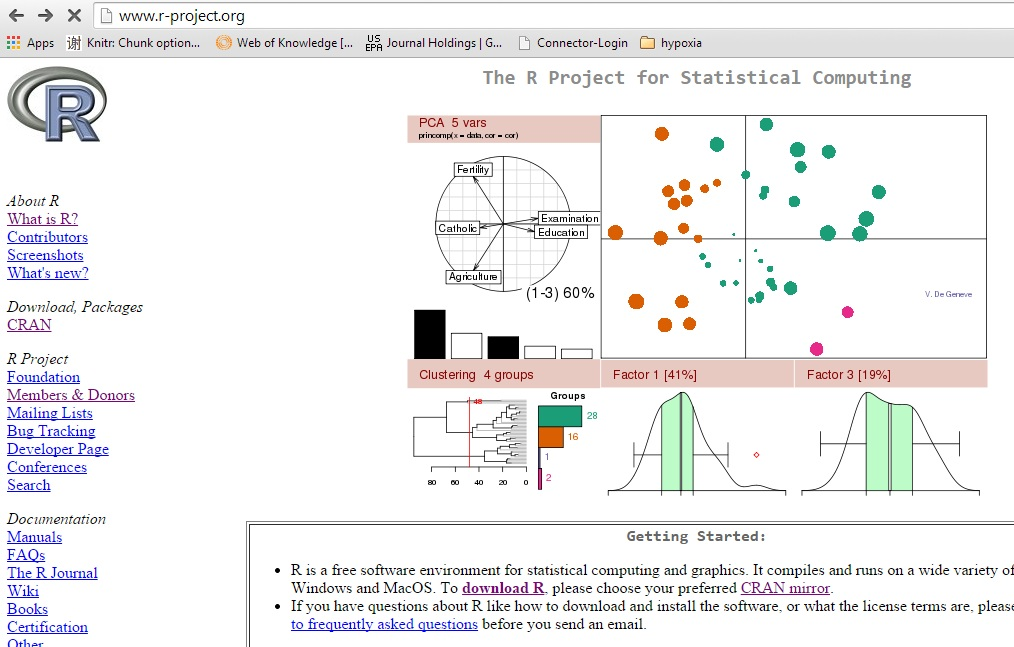
\includegraphics[width=0.8\textwidth]{figs/rpage.jpg}

\item{On the main page, select the \href{http://cran.r-project.org/mirrors.html}{CRAN} link from the menu on the left.}

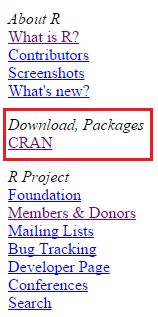
\includegraphics[width=0.2\textwidth]{figs/cransel.png}

\item{Select a mirror from which the R files will be downloaded.  It is best to choose a location that is closest to you.}

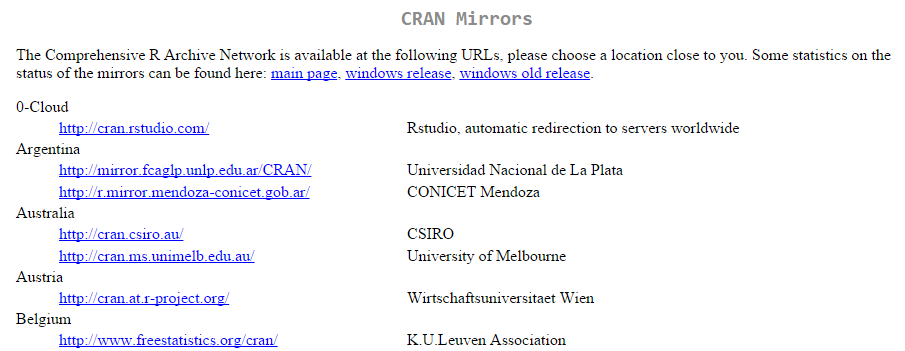
\includegraphics[width=0.8\textwidth]{figs/mirrors.png}

\item{Select the installation option for your operating system.}

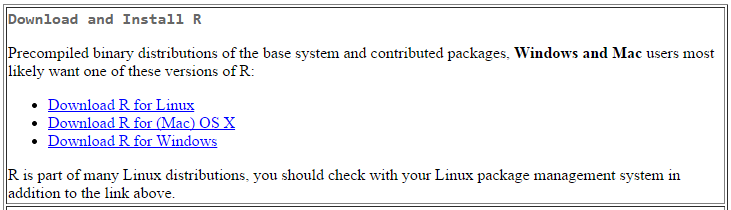
\includegraphics[width=0.8\textwidth]{figs/installos.png}

\item{Select the base option if this is your first time installing R.  The contrib option is a link to the source code for all available packages, which can be installed later from within R.}

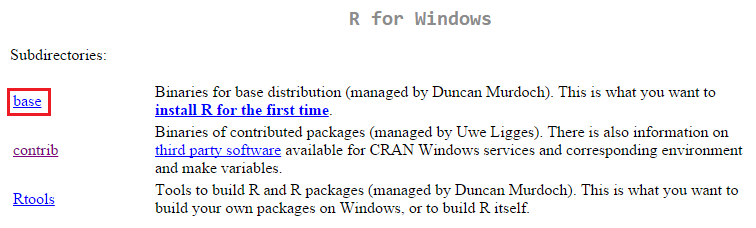
\includegraphics[width=0.8\textwidth]{figs/base.png}

\item{Select the download link. A .exe file will be downloaded to the default download location for your computer.}

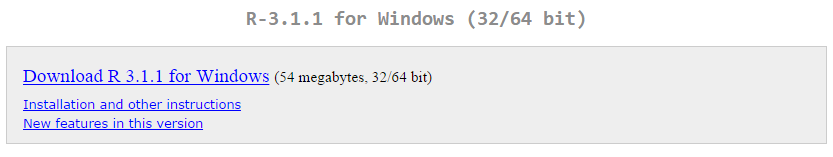
\includegraphics[width=0.8\textwidth]{figs/download.png}

\item{Locate the .exe file that you just downloaded and double-click to begin installation.  It should be named `R-3.1.1\_win.exe' or something similar.}

\item{Follow the installation instructions.  This step may require administration rights.}

\item{A few points are worth mentioning during the installation process:}

\begin{itemize}

\item{You will be prompted to select an installation path for R.  It is best to choose a folder for which you have read/write privileges.  You may wish to change some of the settings for R at a later date, and this is easiest if R is installed in a folder that you can access.}

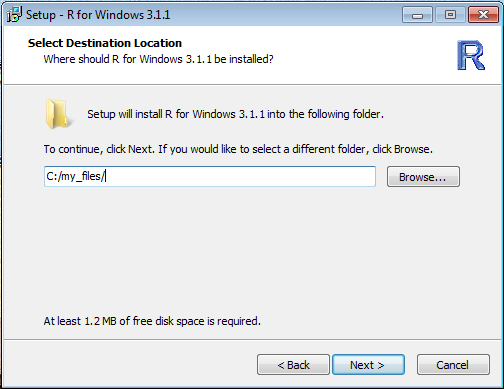
\includegraphics[width=0.7\textwidth]{figs/local.png}

\item{You may also wish to customize the startup options for R.  It is fine to select the defaults, but you may want to tailor the options based on your preferences.}

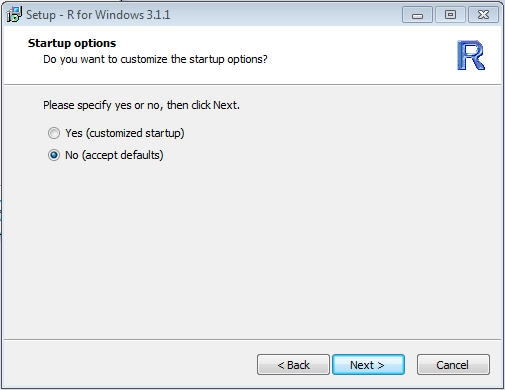
\includegraphics[width=0.7\textwidth]{figs/custom.png}

\end{itemize}

\item{You should be able to use R after the installation process is complete.  We will cover R basics at a later date.}

\end{enumerate}

\section{Installing RStudio - optional}

\href{http://www.rstudio.com/}{RStudio} is an Integrated Development Environment (IDE) that allows for easier use of R and access to additional features for improving functionality. Although it is not necessary for using R, we strongly encourage installation to improve your experience with this software.  General features include a user console, syntax-highlighting edtitor that supports direct code execution, as well as tools for plotting, history, debugging, and workspace management.  Like R, it is also open-source and available as a free download.  An RStudio installation will recognize R if it is previously installed.  As before, installation requires administration privileges. The following is a step-by-step guide to installing RStudio:

\begin{enumerate}

\item{Visit the RStudio website using a web browser: \href{http://www.rstudio.com}{www.rstudio.com}.  Click on the \href{http://www.rstudio.com/products/RStudio/}{Download RStudio} link.}

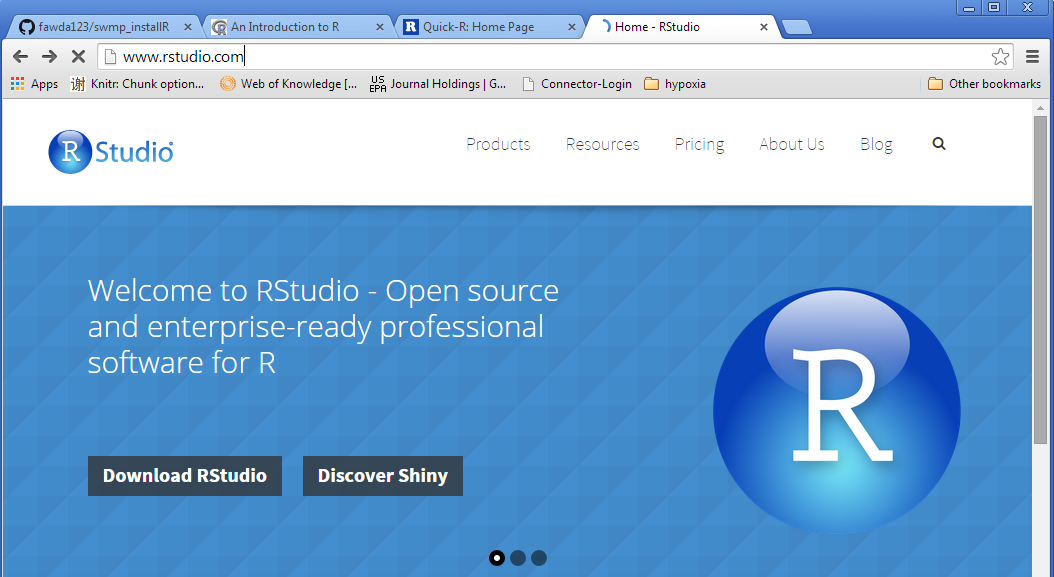
\includegraphics[width=0.8\textwidth]{figs/rstudio.png}

\item{Click on the \href{http://www.rstudio.com/products/RStudio/#Desk}{Desktop} link}

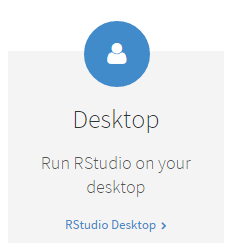
\includegraphics[width=0.3\textwidth]{figs/desktop.png}

\item{Click on the \href{http://www.rstudio.com/products/rstudio/download/}{Download RStudio Desktop} link}

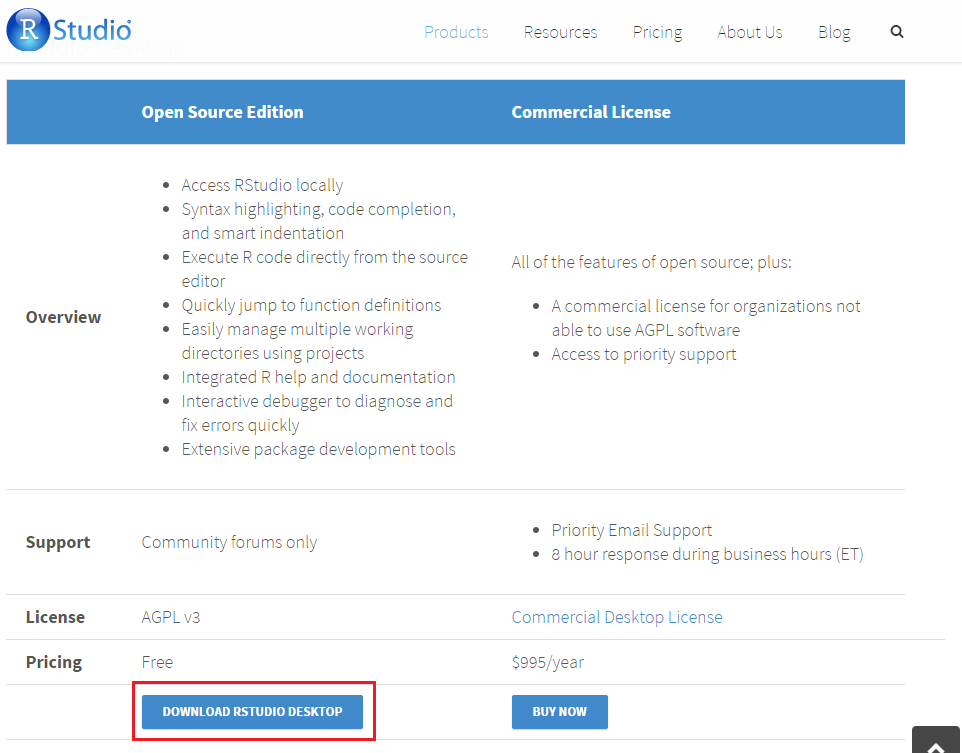
\includegraphics[width=0.8\textwidth]{figs/downloadrstudio.png}

\item{Click the link for your operating system.  A .exe file will be downloaded to the default download location for your computer.}

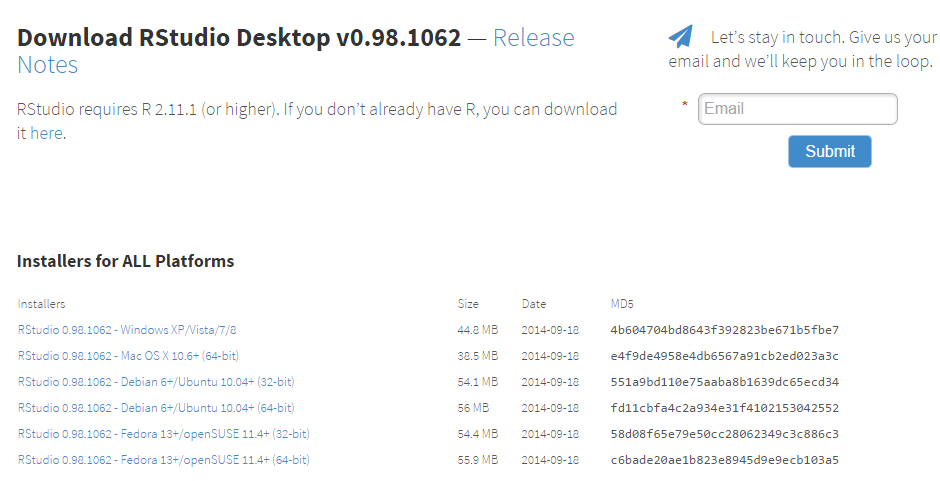
\includegraphics[width=0.8\textwidth]{figs/installosrstudio.png}

\item{Locate the .exe file that you just downloaded and double-click to begin installation.  It should be named `RStudio-0.98.1062.exe' or something similar.  This step requires administration rights.}

\item{Follow the installation instructions.}

\item{Once complete, you should have a working version of RStudio that you can use with R.}

\end{enumerate}

\end{document}
